\subsection{Overview}\label{subsec:overview}
\paragraph{}
An alternative to the security patch it would also be possible to re-write the entire application to not only remedy the addressed
security issues but also make improvements to a few key traits.

\subsubsection{Core Requirements}\label{subsubsec:core-goals}
\paragraph{}
There are few core requirements that are the pillars of the application.
Again they are only touched upon for brevity, thus I would be happy to explain them further at request.

\paragraph{Offline First (PWA) - \emph{Optional}}\label{para:pwa}
Unfortunately it would be unrealistic to assume that the mobile users of the application would have a good connection to the internet at all times.
Whether it is a job in a location where reception is not reliable or a network outage the application would need to handle situations where
it expects to not have instantaneous access to a server.
This is where \href{https://web.dev/progressive-web-apps/}{\textbf{Progression Web Apps (PWA's)}} strive.
It is important to note that functionality would be limited whilst offline leading to an increased development cost.
As a result I have separately quoted this feature.

\paragraph{Limited Data Transfers}
As the application UI would be a single page application we can limit the data transferred from the server.
There would be an increased load time for the initial application to download the static assets and general UI that is then cached for
later use.
With that in place the only data required from the server would be dynamic data such as user jobs.
This data would be transferred in a minimal format such as JSON in which the application would render suitable components.

\paragraph{Purpose Driven UI Navigation}
As there is a varied user base it is important for functionality to be clear and flow in a way that allows the user
to achieve what they need naturally without the need to translate the real life task into the applications' workflow.
\begin{description}
    \item \emph{Limit Paths:} Although it may sound counter-intuitive it is important to limit the paths that a user can take through
    an application.
    This not only makes the process clear for the user but also gives management an easy measure to reflect the correct process.
    \item \emph{Relevant Elements and Reducing Page Jumps:} It is important that elements and information required for tasks is presented or easily accessible to the user.

    \item \emph{Mobile Friendly:} As the majority of users would be using a mobile device it is important that the application is optimised
    to be used on mobile devices.
\end{description}

For a clear example it would be worth looking at the prototype page \href{https://cpr.caleb-dunn.tech/jsheet/5116}{\textbf{HERE}}.

\paragraph{Resource Efficient and Scalable}
It is ultimately the goal of any software to be resource efficient, fast and scalable but to achieve this the software architecture must be
thoughtfully planned out.
By using appropriate and fast technologies / languages for certain sections of the application allow for using the right tool for the job.
The proposed design aims to separate layers of the application that would allow for more instances to be spun up although this would
likely not be needed due to the scope of the application.

\paragraph{Native Application Potential}
Whilst a native mobile application is not included in the software package it would be possible to implement a technology like \href{https://reactnative.dev/}{\textbf{React Native}} to
develop a native mobile application that could be installed onto devices whilst leveraging the existing code for the website.
This would be more robust than the \hyperref[para:pwa]{\textbf{PWA}} but would require more development.

\subsubsection{General Application Flow}
\paragraph{}
Below is an example of how a user authenticates and interacts with the application and how the components interact with each other.

\paragraph{Assumption}
User has an account and has already visited the website and downloaded required assets.
\begin{enumerate}
    \item User Login
    \begin{enumerate}
        \item User enters login credentials on login page.
        \item Credentials are sent to GO webserver through Caddy proxy.
        \item GO webserver retrieves user details from PostgreSQL matched on username.
        \item Compute password hash for password sent to server and compare with the existing stored hash. \emph{If invalid user is notified and re-prompted to login.}
        \item Generate and set access token for user session in Redis and as a client cookie.
    \end{enumerate}
    \item User navigates to current jobs.
    \begin{enumerate}
        \item Using access token in cookie a request is sent to the webserver.
        \item The webserver uses the access token to retrieve the user session from Redis.
        \item If the access token and user session is valid the webserver requests the users job data from PostgreSQL.
        \item Webserver serialises jobs into JSON and sends back to user.
        \item User receives jobs to interact with.
    \end{enumerate}
\end{enumerate}


\pagebreak

\subsubsection{General Data Request Example}
\paragraph{}

\begin{figure}[h!]
    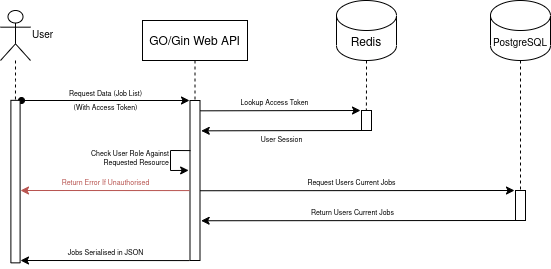
\includegraphics[width=\textwidth]{res/general-api-request}
    \caption{A generic job data retrieval}
    \label{fig:general-api-req}
\end{figure}

\pagebreak
\subsection{Major Components}\label{subsec:major-components}
The application is broken into several applications that specialise at given tasks to drastically reduce development time
and increase performance.
This section provides a brief explanation of the technology and why it was chosen.

\begin{figure}[h!]
    \includegraphics[width=\textwidth]{res/general_data_flow}
    \caption{How components interact}
    \label{fig:how-services-interact}
\end{figure}

\subsubsection{ReactJS Front End}
\paragraph{}
ReactJS is a JavaScript framework created and backed by Facebook that drastically simplifies and empowers the creation of Single Page Applications \emph{SPA's} in the
web browser.
This will be the technology that a user will interface with when using the CPR application.
An SPA means that the page will be fully loaded once with every other action  swapping out parts of the web page instead of
an entire page refresh/rerender.
It is important to note that the rendering takes place on the user's device and not the server.

\paragraph{Mobile First}
ReactJS has a useful UI/Component library \textbf{\href{https://mui.com/}{(MUI)}} prioritises mobile first applications.
This approach means that mobile devices are priority platform for development and UI's for desktop are scaled up / modified after.
This is vital as the majority of users will be on mobile devices that have limited screen space and input options when compared
to desktop devices.

\paragraph{Data Usage Reduction}
As the SPA renders on the client it only needs the raw data in order to create a meaningful UI with dynamic data.
Instead of requesting an entire pre rendered job page it is possible to only request the raw job data that can be parsed
by React to minimise user-server communication and data.

\paragraph{PWA Support}
ReactJS's SPA nature simplifies the creation of a PWA for device installation and offline first behaviour.
Although it is not strictly a React feature it saves development time.

\paragraph{Community and Third Party Libraries}
ReactJS has an enormous and active community with lots of Facebook support meaning it is not likely to go away anytime soon.
With the huge community there are tens of thousands of third party libraries that extend React functionalities for virtually any
scenario.

\paragraph{React Native Extension} If CPR wants a native application for mobile devices a large majority of the existing codebase
could be used, thus reducing development time significantly.
Having developed an enterprise application using React Native I believe it would be a suitable option if the need arises.


\paragraph{} ReactJS Documentation: \url{https://reactjs.org/docs/getting-started.html}

\subsubsection{GO Gin REST API}
\paragraph{}
At the core of the application is a REST API written in GO using the Gin framework.
Traffic will go through a web server proxy like Caddy to abstract HTTPS and static file delivery.

\paragraph{GO Summary}
GO is a modern compiled language created by Google with the purpose of being simple and easy to learn with a strong concurrency model.
This purpose fulfils CPR's requirements with its backend service as it's simplicity allows for ad-hoc future development and by nature web services
are concurrent in nature serving multiple users at a given time.

\paragraph{} GO Documentation: \url{https://go.dev/doc/}

\paragraph{Gin Summary}
Gin is a HTTP framework that abstracts away from lower level \href{https://pkg.go.dev/net/http}{http} package leading to a monumental decrease
in complexity and development time.
Gin leverages of GO's goroutines to serve each request concurrently whilst maintaining the simplicity of single threaded programming.

\paragraph{} Gin Documentation: \url{https://github.com/gin-gonic/gin}



\subsubsection{Caddy Web Server}
\paragraph{}
Caddy is a new open source web server that can be used to proxy communication from the user to the GO web API alongside static
content like images.
What makes Caddy unique is that it automatically configures HTTPS for websites using LetsEncrypt or zeroSSL with no configuration
needed at all.
It is truly set and forget.

\paragraph{}
Apache httpd could be used instead of Caddy, however it would require configuration for SSL.

\paragraph{} Caddy Documentation: \url{https://caddyserver.com/docs/}

\subsubsection{PostgreSQL Database}
PostgreSQL is an open source object-relational database that is reliable and performant.
For an application of this scale the decision between the common database options becomes one of preference.
I like using PostgreSQL as it comes with native support for quality of life features such as UUID's.

\paragraph{MySQL}
I have noticed the current application use MySQL as its database.
Postgres is virtually better than MySQL in every facet, from developer experience to performance.
MySQL is a legacy product that has very specific use cases.

\paragraph{GO PostgreSQL Drivers}
There are a multitude of a PostgreSQL driver libraries available in GO meaning that development time is saved with arguably
better performance.

\paragraph{} PostgreSQL Documentation: \url{https://www.postgresql.org/docs/}

\subsubsection{Redis Session Cache}
\paragraph{}
Redis is an in-memory database designed for quick access and caching.
Using keys to hash and store data we can use it for user session management and authentication in a fast and resource efficient
manner.
Redis has the ability to set an expiry for all data types, thus allowing access tokens to have an insured lifetime which is
extremely important with short-lived tokens.

\paragraph{} In the future, it would be possible to cache other data like users jobs to avoid a round trip to the PostgreSQL
database however, this would be overkill at this current time.

\begin{figure}[h!]
    \begin{center}
    \fbox{%
    \begin{minipage}{0.8\textwidth}%
        \textcolor{gray}{Create a session instance using session-token as key} \\
        HSET \textcolor{violet}{mykey} \textcolor{purple}{user} LC1  \textcolor{purple}{role} admin \\
        \textcolor{gray}{Set key to expire after 60 seconds} \\
        EXPIRE \textcolor{violet}{mykey} 60 \\
        \textcolor{gray}{Get values in key} \\
        HGETALL \textcolor{violet}{mykey}
    \end{minipage}
    }
    \caption{Creating, storing and fetching a user session in Redis}
    \label{fig:example-session-use}
    \end{center}
\end{figure}

\paragraph{} Redis Documentation: \url{https://redis.io/documentation}

\subsection{Advantages vs Implementing Security in Existing System}\label{subsec:advantages-vs-implementing-security-in-existing-system}

\paragraph{Unforeseen Security Vulnerabilities} The complete software package includes all the security features above one is not more secure than the other.
It is important to note however that I have not seen the existing codebase so there may be security risks that I have not seen from
a preliminary look from the outside.
An example of such an attack could be incorrectly validated data inputs causing a multitude of potential attack vectors such as
SQL injection, remote code execution or cross site scripting.

\paragraph{}
Advantages can be reflected in the core requirements and their implementations explained above, but personally I feel the biggest
advantage comes with the User Interface and User Experience improvements.
I have supplied an informal supplementary document that highlight some proposed usability changes present in the current prototype.

\clearpage
\printglossaries